\documentclass{article} 
\usepackage{graphicx}
\usepackage[spanish]{babel}
\usepackage[autostyle]{csquotes}
\usepackage{tabto}
\usepackage{booktabs}

\renewcommand{\contentsname}{Contenido}
\renewcommand{\figurename}{Im\'agen}


% \newcommand{\itab}[1]{\hspace{0em}\rlap{#1}}
% \newcommand{\tab}[1]{\hspace{.05\textwidth}\rlap{#1}}

\title{Proyecto 3\\Traductores} 
\author{Samuel Arleo\and Sergio Ter\'an } 
\date{06 Marzo, 2016}

\begin{document}

	%Portada
		\pagenumbering{gobble}
		\begin{center}
		 	\pagestyle{headings} \small
		 	
\includegraphics[scale=0.4]{USB.png}\\[0.3cm]
			Universidad Sim\'on Bolivar\\[0.1cm]
		 	Departamento de Computaci\'on y Tecnolog\'ia de la Informaci\'on\\[0.1cm]
		 	CI3725 - Traductores e Interpretadores\\[0.1cm]
		 	Enero-Marzo 2016\\[0.1cm]

			\vspace{15em}
			\LARGE Proyecto 3\\
			\vspace{0.5em}
			\Large Traductores\\
			\vspace{0.5em}
			\large Samuel Arleo \-\hspace{5em}Sergio Ter\'an\\
			\vspace{0.5em}
			\large 10-10969 \-\hspace{7em}11-11020\\
			\vspace{15em}
			07 de Marzo, 2016
		\end{center}

	%Seccion sobre la implementacion
		\newpage
		\pagenumbering{arabic}
		\section{Formulaci\'on e Implementaci\'on} 
Para realizar el an\'alisis sem\'antico del lenguaje BOT se utiliz\'o la noci\'on de gram\'atica de atributos, ya que se empleo una variable global “tabla” (atributo heredado). Fueron necesarios algunos ajustes en la gram\'atica e implementar nuevas estructuras de datos tales como la clase “pila”, “datos” y “tabla”. Algunas de las decisiones de diseño fueron:
\\
\begin{enumerate}
\item[*] Todas las variables declaradas dentro de la lista de comportamientos de un robot poseen el mismo tipo del robot (incluyendo a la variable asociada al robot “me”)
\item[*] La variable asociada al robot “me” es distinta para cada robot, así la declaraci\'on pudiera haber sido hecha con una lista de robots.
\item[*] Las el numero de instrucciones de robot “default” puede ser maximo 1 para cada robot.
\item[*] Una instrucci\'on de robot “activation” / ”deactivation” no puede aparecer dos veces seguidas en una lista de comportamientos.
\item[*] Una instrucci\'on de robot “activation” no puede ocurrir luego de otro “activation”
\item[*] Una instrucci\'on de robot “deactivation” no puede ocurrir luego de otro “deactivation”
\item[*] La aceptaci\'on de expresiones de la forma `a' = `b' fue realizada utilizando la gram\'atica, por lo que un error en este tipo de expresiones sera visto como un error sint\'actico.
* Las incorporaciones de alcance contaran con el acceso a las variables declaradas en los niveles superiores
\end{enumerate}
	%Seccion de respuestas teorico practicas
		\newpage
		\section{Revisi\'on Te\'orico-Practica}
			\begin{enumerate}
				%Pregunta 1
				\large \bf \item[] Pregunta 1
				\normalsize \mdseries
					\begin{enumerate}
					%Parte (a)
					\item[(a)] \
						\begin{enumerate}
							\item[(a.1)] 
								$G_{1}$ = (\{S\},\{a\},\{S $\longrightarrow$ Sa,S $\longrightarrow$ $\lambda$\},S)\\
								\\
								Determinemos si la gram\'atica\\
								\begin{tabbing}
								\hspace*{2cm} \= \hspace*{0.6cm} \= \hspace*{3cm} \kill
									%p_inicio
									\>S \' $\longrightarrow$\> Sa\\
									\>S \' $\longrightarrow$\> $\lambda$\\
								\end{tabbing}
								Es LR(1) y construyamos su analizador sint\'actico. 
								Comenzamos por aumentar la gramatica con el s\'imbolo $S^{\prime}$ y agregando el s\'imbolo \$ al final de la primera entrega. A dem\'as enumeramos las producciones.
								\begin{tabbing}
								\hspace*{1cm} \= \hspace*{1cm} \= \hspace*{1cm} \= \hspace*{0.6cm} \= \hspace*{0.6cm} \= \hspace*{3cm} \kill
									%item 0
									\> (i)\>  $S^{\prime}$	\> $\longrightarrow$\> 	S\$ 	\\
									\> (ii)\>  $S$	\> $\longrightarrow$\> 	Sa 	\\
									\> (iii)\>  $S$	\> $\longrightarrow$\>  $\lambda$ 	\\
								\end{tabbing}
								Construimos los conjuntos FIRST y FOLLOW para los simbolos no terminales:
								\begin{quotation}
									FIRST($S^{\prime}$) = \{ $\lambda$ , a \}
								\end{quotation}
								\begin{quotation}
									FIRST($S$) = \{ $\lambda$ , a \}
								\end{quotation}
								\begin{quotation}
									FOLLOW($S^{\prime}$) = \{ \$ \}
								\end{quotation}
								\begin{quotation}
									FOLLOW($S$) = \{ a, \$ \}
								\end{quotation}
								El conjunto de clauduras nos queda:\\
								\begin{tabbing}
								 \hspace*{1cm} \= \hspace*{1cm} \= \hspace*{0.6cm} \= \hspace*{0.6cm} \= \hspace*{3cm} \kill
									%item 0
									\> $I_{0}$	\' : 	\> $S^{\prime}$	\> $\longrightarrow$\> 	$\cdot$S\$ 	\\
									\>		\'  	\> $S$ 			\> $\longrightarrow$\> 	$\cdot$Sa 	\\
									\>		\'  	\> $S$ 			\> $\longrightarrow$\> 	$\cdot$ 	\\
								
									%item 1
									\>$I_{1}$	\' : 	\> $S^{\prime}$ \> $\longrightarrow$\> 	S$\cdot$\$	\\
									\>		\'  	\> $S$ 			\> $\longrightarrow$\> 	S$\cdot$a	\\
									
									%item 2
									\>$I_{2}$	\' : 	\> $S^{\prime}$ \> $\longrightarrow$\> 	S\$$\cdot$	\\
									
									%item 3
									\>$I_{3}$	\' : 	\> $S$ 			\> $\longrightarrow$\> 	Sa$\cdot$	\\
								\end{tabbing}
								Construimos el automata de prefijos viables, que nos queda de la forma:\\
				 				
							  		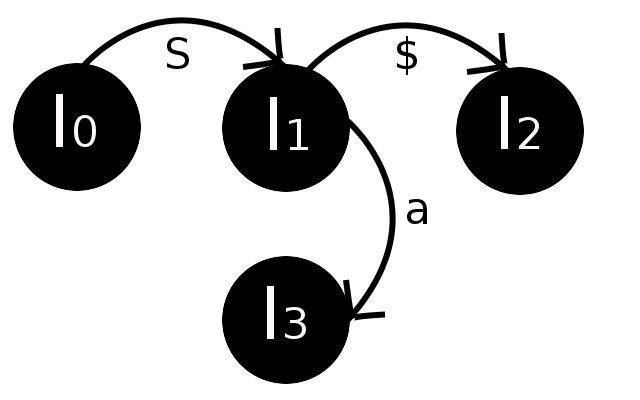
\includegraphics[ scale=0.2]{grafo1.png}
							  	\\Ahora podemos constriur la tabla de parsing $SLR(1)$:
							  	\\
				 				\begin{tabular}{l | c c | c c}
									\toprule
									&\multicolumn{2}{|c|}{Acciones} &\multicolumn{2}{|c}{Goto}\\
									\midrule[0.5mm]
									& a & \$ & $S^{\prime}$ & S \\
									\midrule[0.5mm]
										$I_{0}$ & r(iii) & r(iii) &  & 1 \\
									\hline
										$I_{1}$ & s(3) & s(2) &  &  \\
									\hline
										$I_{2}$ &  & $acc$ &  &  \\
									\hline
										$I_{3}$ & r(ii) & r(ii) &  &  \\
									\bottomrule
								\end{tabular}
							\\\\\
							\item[(a.2)] 
								$G_{1}$ = (\{S\},\{a\},\{S $\longrightarrow$ aS,S $\longrightarrow$ $\lambda$\},S)\\
								\\
								Determinemos si la gram\'atica\\
								\begin{tabbing}
								\hspace*{2cm} \= \hspace*{0.6cm} \= \hspace*{3cm} \kill
									%p_inicio
									\>S \' $\longrightarrow$\> aS\\
									\>S \' $\longrightarrow$\> $\lambda$\\
								\end{tabbing}
								Es LR(1) y construyamos su analizador sint\'actico. 
								Comenzamos por aumentar la gramatica con el s\'imbolo $S^{\prime}$ y agregando el s\'imbolo \$ al final de la primera entrega. A dem\'as enumeramos las producciones.
								\begin{tabbing}
								\hspace*{1cm} \= \hspace*{1cm} \= \hspace*{1cm} \= \hspace*{0.6cm} \= \hspace*{0.6cm} \= \hspace*{3cm} \kill
									%item 0
									\> (i)\>  $S^{\prime}$	\> $\longrightarrow$\> 	S\$ 	\\
									\> (ii)\>  $S$	\> $\longrightarrow$\> 	aS 	\\
									\> (iii)\>  $S$	\> $\longrightarrow$\>  $\lambda$ 	\\
								\end{tabbing}
								Construimos los conjuntos FIRST y FOLLOW para los simbolos no terminales:
								\begin{quotation}
									FIRST($S^{\prime}$) =  FIRST($S$) = \{ $\lambda$ , a \}
								\end{quotation}

								\begin{quotation}
									FOLLOW($S^{\prime}$) =  FOLLOW($S$) = \{ \$ \}
								\end{quotation}

								El conjunto de clauduras nos queda:\\
								\begin{tabbing}
								 \hspace*{1cm} \= \hspace*{1cm} \= \hspace*{0.6cm} \= \hspace*{0.6cm} \= \hspace*{3cm} \kill
									%item 0
									\> $I_{0}$	\' : 	\> $S^{\prime}$	\> $\longrightarrow$\> 	$\cdot$S\$ 	\\
									\>		\'  	\> $S$ 			\> $\longrightarrow$\> 	$\cdot$aS 	\\
									\>		\'  	\> $S$ 			\> $\longrightarrow$\> 	$\cdot$ 	\\
								
									%item 1
									\>$I_{1}$	\' : 	\> $S^{\prime}$ \> $\longrightarrow$\> 	S$\cdot$\$	\\
									
									%item 2
									\>$I_{2}$	\' : 	\> $S$ \> $\longrightarrow$\> 	a$\cdot$S	\\
									\>			\'  	\> $S$ \> $\longrightarrow$\> 	$\cdot$aS	\\
									\>			\'  	\> $S$ \> $\longrightarrow$\> 	$\cdot$	\\
									
									%item 3
									\>$I_{3}$	\' : 	\> $S$ 			\> $\longrightarrow$\> 	aS$\cdot$	\\

									%item 4
									\>$I_{4}$	\' : 	\> $S^{\prime}$	\> $\longrightarrow$\> 	S\$ $\cdot$	\\
								\end{tabbing}
								Construimos el automata de prefijos viables, que nos queda de la forma:\\
				 				
							  		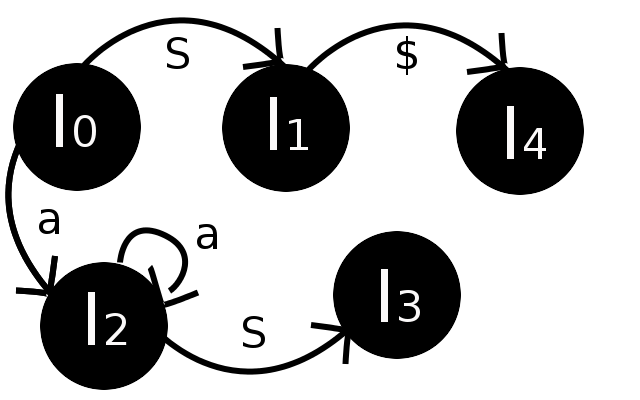
\includegraphics[ scale=0.2]{grafo2.png}
							  	\\Ahora podemos constriur la tabla de parsing $SLR(1)$:
							  	\\
				 				\begin{tabular}{l | c c | c c}
									\toprule
									&\multicolumn{2}{|c|}{Acciones} &\multicolumn{2}{|c}{Goto}\\
									% &Acciones& &GoTo\\
									\midrule[0.5mm]
									& a & \$ & $S^{\prime}$ & S \\
									\midrule[0.5mm]
										$I_{0}$ & s(2) & r(iii) &  & 1 \\
									\hline
										$I_{1}$ &  & s(4) &  &  \\
									\hline
										$I_{2}$ & s(2) & r(iii) &  & 3 \\
									\hline
										$I_{3}$ &  & r(ii) &  &  \\
									\hline
										$I_{4}$ &  & $acc$ &  &  \\
									\bottomrule
								\end{tabular}


						\end{enumerate}
					%Parte (b)
					\item[(b)] Comparando las tablas de $G1_{i}$ y $G1_{d}$ vemos que la tabla de parsing de $G1_{i}$ contiene menos filas que $G1_{d}$. 
					\\\\
					En la pila, $G1_{i}$, consume un maximo de 3 items en la pila, en el caso especifico de la frase $aaa$ la pila  para $G1_{d}$ puede llegar a tener hasta 4 items, por lo que podemos ver que $G1_{i}$ es mas eficiente en cuanto al consumo de memoria por parte de la pila.
					\\\\
					a dem\'as vemos que para reconocer las frases, la cantidad de movimientos realizados por ambos es de $2*n+3$ po lo que el tiempo de ejecucion es de orden $O(n)$ donde $n$ es la cantidad de `a' en la frase.
					\\\\ 

					
					\end{enumerate}
				\large \bf \item[] Pregunta 2
				\normalsize \mdseries
					\begin{enumerate}
					%Parte (a)
					\item[(a)]								
					\begin{tabbing}
								\hspace*{1cm} \= \hspace*{1cm} \= \hspace*{1cm} \= \hspace*{0.6cm} \= \hspace*{0.6cm} \= \hspace*{3cm} \kill
									\> (i)\>  $S^{\prime}$	\> $\longrightarrow$\> 	$Instr$ 	\\
									\> (ii)\>  $Instr$	\> $\longrightarrow$\> 	$Instr$ ; $Instr$ 	\\
									\> (iii)\>  $Instr$	\> $\longrightarrow$\>  IS 	\\
					\end{tabbing}
					\begin{quotation}
						FIRST($S^{\prime}$) =  FIRST($Instr$) = \{ IS \}
					\end{quotation}		
					\begin{quotation}
						FOLLOW($S^{\prime}$) \{ \$ \}
					\end{quotation}
					\begin{quotation}
						FOLLOW($Instr$) \{ ;,\$ , IS \}
					\end{quotation}						
					\ \ 
					\begin{tabbing}
					 \hspace*{1cm} \= \hspace*{1cm} \= \hspace*{0.8cm} \= \hspace*{0.6cm} \= \hspace*{3cm} \kill
						%item 0
						\> $I_{0}$	\' : 	\> $S^{\prime}$		\> $\longrightarrow$\> 	$\cdot Instr$ \$	\\
						\>			\'  	\> $Instr$ 			\> $\longrightarrow$\> 	$\cdot Insrr$ ; $Instr$	\\
						\>			\'  	\> $Instr$ 			\> $\longrightarrow$\> 	$\cdot$ IS	\\


						%item 1
						\> $I_{1}$	\' : 	\> $S^{\prime}$		\> $\longrightarrow$\> 	$Instr \cdot$ \$	\\
						\>			\'  	\> $Instr$ 			\> $\longrightarrow$\> 	$Instr \cdot$ ; $Instr$	\\

						%item 2
						\>$I_{2}$	\' : 	\> $Instr$ 			\> $\longrightarrow$\> 	IS$\cdot$	\\

						%item 3
						\>$I_{3}$	\' : 	\> $S^{\prime}$		\> $\longrightarrow$\> 	$Instr$\$$\cdot$	\\

						%item 4
						\>$I_{4}$	\' : 	\> $Instr$			\> $\longrightarrow$\> 	$Instr$ ; $\cdot$ $Instr$	\\
						\>			\'  	\> $Instr$ 			\> $\longrightarrow$\> 	$\cdot Instr$ ; $Instr$	\\
						\>			\'  	\> $Instr$ 			\> $\longrightarrow$\> 	$\cdot$IS	\\

						%item 5
						\>$I_{5}$	\' : 	\> $Instr$			\> $\longrightarrow$\> 	$Instr$ ; $Instr$ $\cdot$	\\
						\>			\'  	\> $Instr$ 			\> $\longrightarrow$\> 	$Instr \cdot$ ; $Instr$	\\
					\end{tabbing}

					En la regla $I_{5}$ vemos que existe un conflicto 
					\
					\\
					%Parte (b)
					\item[(b)]Este conflicto, del tipo $shift/reduce$, lo intentaremos solucionar usando el algoritmo de SLR(1), apoyandonos con los FIRST y FOLLOW que ya hemos calculado.
	 				\\\\\
	 				\begin{tabular}{l | c c c | c c}
						\toprule
						&\multicolumn{3}{|c|}{Acciones} &\multicolumn{2}{|c}{Goto}\\
						% &Acciones& &GoTo\\
						\midrule[0.5mm]
						& ; & IS & \$ & $S^{\prime}$ & $Instr$ \\
						\midrule[0.5mm]
							$I_{0}$ &  & s(2) &  &  & 1 \\
						\hline
							$I_{1}$ & s(4) &  & s(3) &  \\
						\hline
							$I_{2}$ & r(iii) & r(iii) & r(iii) &  \\
						\hline
							$I_{3}$ &  &  & $acc$ &  \\
						\hline
							$I_{4}$ &  & s(2) &  &  \\
						\hline
							$I_{4}$ & \textbf{s(4)/r(ii)} & r(ii) & r(ii) &  \\
						\bottomrule
					\end{tabular}
					\ 
					\\\\
					%Parte (c)
					\item[(c)]
					Secuencia de reconocimiento para la frase IS;IS;IS, dando prioridad al $shift$ en el conflicto $shift/reduce$
					\ 
					\\\\
					\begin{tabular}{|c|c|c|c|}
						\hline
						Pila & Entrada & Acci\'on & Salida\\	
						\hline
						$I_{0}$ & IS;IS;IS\$ & s(2) &
						\\
						\hline
						$I_{2}$
						$I_{0}$ & ;IS;IS\$ & r(iii) &
						(iii)\\
						\hline
						$I_{1}$
						$I_{0}$ & ;IS;IS\$ & s(4) &
						(iii)\\
						\hline
						$I_{4}$
						$I_{1}$
						$I_{0}$ & IS;IS\$ & s(2) &
						(iii)\\
						\hline
						$I_{2}$
						$I_{4}$
						$I_{1}$
						$I_{0}$ & ;IS\$ & r(iii) &
						(iii),
						(iii)\\
						\hline
						$I_{5}$
						$I_{4}$
						$I_{1}$
						$I_{0}$ & ;IS\$ & s(4) &
						(iii),
						(iii)\\
						\hline
						$I_{4}$
						$I_{5}$
						$I_{4}$
						$I_{1}$
						$I_{0}$ & IS\$ & s(2) &
						(iii),
						(iii)\\
						\hline
						$I_{2}$
						$I_{4}$
						$I_{5}$
						$I_{4}$
						$I_{1}$
						$I_{0}$ & \$ & r(iii) &
						(iii),
						(iii),
						(iii)\\
						\hline
						$I_{5}$
						$I_{4}$
						$I_{5}$
						$I_{4}$
						$I_{1}$
						$I_{0}$ & \$ & r(ii) &
						(ii),
						(iii),
						(iii),
						(iii)\\
						\hline
						$I_{5}$
						$I_{4}$
						$I_{1}$
						$I_{0}$ & \$ & r(ii) &
						(ii),
						(ii),
						(iii),
						(iii),
						(iii),\\
						\hline
						$I_{1}$
						$I_{0}$ & \$ & s(3) &
						(ii),
						(ii),
						(iii),
						(iii),
						(iii),\\
						\hline
						$I_{3}$
						$I_{1}$
						$I_{0}$ & \$ & $acc$ &
						(ii),
						(ii),
						(iii),
						(iii),
						(iii),\\
						\hline

					\end{tabular}
					% \newpage
					\\
					\\
					\\Secuencia de reconocimiento para la frase IS;IS;IS, dando prioridad al $reduce$ en el conflicto $shift/reduce$\\

					\begin{tabular}{|c|c|c|c|}
						\hline
						Pila & Entrada & Acci\'on & Salida\\	
						\hline
						$I_{0}$ & IS;IS;IS\$ & s(2) &
						\\
						\hline
						$I_{2}$
						$I_{0}$ & ;IS;IS\$ & r(iii) & 
						(iii)\\
						\hline
						$I_{1}$
						$I_{0}$ & ;IS;IS\$ & s(4) & 
						(iii)\\
						\hline
						$I_{4}$
						$I_{1}$
						$I_{0}$ & IS;IS\$ & s(2) & 
						(iii)\\
						\hline
						$I_{2}$
						$I_{4}$
						$I_{1}$
						$I_{0}$ & ;IS\$ & r(iii) & 
						(iii),
						(iii) \\
						\hline
						$I_{5}$
						$I_{4}$
						$I_{1}$
						$I_{0}$ & ;IS\$ & r(ii) &
						(ii),
						(iii),
						(iii)\\
						\hline
						$I_{1}$
						$I_{0}$ & ;IS\$ & s(4) &
						(ii),
						(iii),
						(iii)\\
						\hline
						$I_{4}$
						$I_{1}$
						$I_{0}$ & IS\$ & s(2) &
						(ii),
						(iii),
						(iii)\\
						\hline
						$I_{2}$
						$I_{4}$
						$I_{1}$
						$I_{0}$ & \$ & r(iii) &
						(iii),
						(ii),
						(iii),
						(iii)\\
						\hline
						$I_{5}$
						$I_{4}$
						$I_{1}$
						$I_{0}$ & \$ & r(ii) &
						(ii),
						(iii),
						(ii),
						(iii),
						(iii)\\
						\hline
						$I_{1}$
						$I_{0}$ & \$ & s(3) &
						(ii),
						(iii),
						(ii),
						(iii),
						(iii)\\
						\hline
						$I_{3}$
						$I_{1}$
						$I_{0}$ & \$ & $acc$ &
						(ii),
						(iii),
						(ii),
						(iii),
						(iii)\\
						\hline
					\end{tabular}
					\
					\\\\
					\\
					Podemos concluir que a pesar de que en ambos casos se genera la misma frase sin asociatividades `explicitas', al priorizar $shift$ nos genera una asociatividad `inplicita' a la izquierda, mientras que al priorizar $reduce$ nos genera una asociatividad `inplicita' a la derecha.
					\\\\
					%Parte (d)
					\item[(d)]
					Para comparar la eficiencia de ambas opciones, reconocimos frase de tamano $IS(;IS)^{2}$, $IS(;IS)^{3}$ , $IS(;IS)^{4}$ y $IS(;IS)^{5}$ para esrudiar sus comportamientos.
					\\\\
					Comparando el comportamiento de las pilas en ambas alternativas, vemos que dando prioridad al $shift$ el tamano maximo de la pila es $2*(n+1)$ para frases de la forma $IS(IS)^{n}$ mientras que para el $reduce$ el tamano maximo de la pila es 4 de manera constante.
					\\\\
					Por otro lado vemos que ambas alternativas cuestan $4(n + 1)$ pasos para aceptar la frase, luego, en cuestion de tiempo  son de orden $O(n)$.
					\\\\
					Podemos concluir que en cuestion de eficiencia la alternativa de $reduce$ es mas conveniente ya que cuesta la misma cantidad de tiempo, pero utiliza menos memoria en su pila.
					\end{enumerate}
									
			\end{enumerate}
\end{document}